\documentclass[10pt,a4paper]{report}
\usepackage[utf8]{inputenc}
\usepackage[T1]{fontenc}
\usepackage{amsmath}
\usepackage{amsfonts}
\usepackage{amssymb}
\usepackage{graphicx}
\usepackage{subfig}
\begin{document}
	\section{Introduction}
	
	\section{WPSL}
	Any rectangle can be fully specified by opposite coordinate of a diagonal fig (\ref{wpsl1}). 
	
	A rectangle of unit area is taken and two ends of the diagonals are $(x_1, y_1)=(0,0)$ and $(x_2, y_2)=(1,1)$. A random point is chosen, say $(x_3, y_3)$. Along with two perpendicular line that random point divides the initial rectangle into four parts labeled as $0,1,2$ and $3$ each with different area. These labels can be considered as nodes and the boundary connecting them as link fig(\ref{wpsl2}).
	Four rectangle will have following diagonal indices starting from \textit{lower left} and going in a counter clockwise manner and increase node number by one at each step
	\begin{align}
		\text{lower left}\quad 0 -> (x_1, y_1) \quad \text{and} \quad (x_3, y_3) \\		
		\text{lower right}\quad 1 -> (x_3, y_1) \quad \text{and} \quad (x_2, y_3) \\
		\text{upper right}\quad 	2 -> (x_3, y_3) \quad \text{and} \quad (x_2, y_2) \\
		\text{upper left}\quad		3 -> (x_1, y_3) \quad \text{and} \quad (x_3, y_2) 
	\end{align}
	
	Figure (\ref{wpsl2}) can be used as a network seed with following adjacency list
	\begin{align}
		0 &: \{1, 3\} \\
		1 &: \{0, 2\} \\
		2 &: \{1, 3\} \\
		3 &: \{0, 2\}
	\end{align}
	\begin{figure}
		\centering
		\subfloat[\label{wpsl1}]{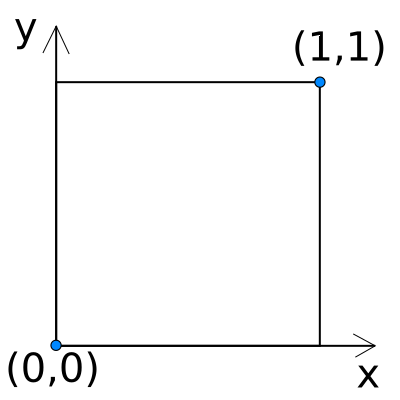
\includegraphics[width=0.6\linewidth]{fig/wpsl1.png}}
		\subfloat[\label{wpsl2}]{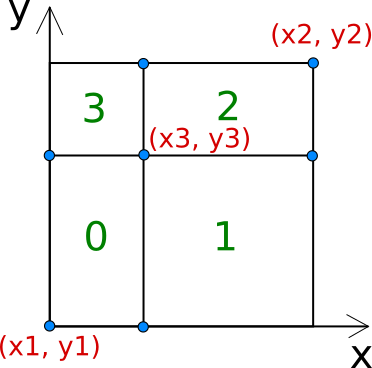
\includegraphics[width=0.6\linewidth]{fig/wpsl2.png}}
		\caption{WPSL. Initial two steps}
	\end{figure}

	Next we choose one of the node randomly (or preferentially with respect to their area, since area can be considered as weight or probability of picking that node). For example we choose node $1$ fig (\ref{wpsl3}). Node $1$ have some neighbors namely $A=\{0, 2\}$.
	
	We take that rectangle and choose a point $(x_4,y_4)$ randomly and divide the rectangle into four parts just like before. Since label $1$ is no longer needed we recycle it by labeling the lower left rectangle by it. Same as before we start from lower left and go on in a counter clockwise manner and increase node number at each step. Note that node $2,3$ is already taken, so we do $1,4,5$ and $6$
	
	\begin{figure}
		\centering
		\subfloat[\label{wpsl3}]{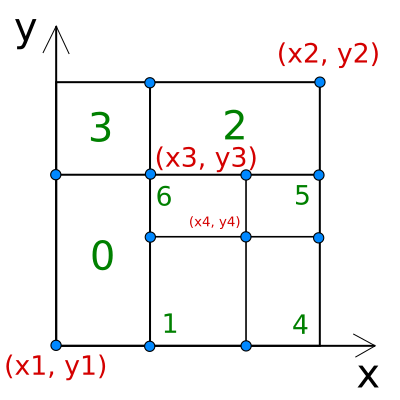
\includegraphics[width=0.8\linewidth]{fig/wpsl3.png}}
		\caption{WPSL. 3rd step.}
	\end{figure}

	\begin{align}
	\text{lower left}\quad 1 -> (x_3, y_1) \quad \text{and} \quad (x_4, y_4) \\		
	\text{lower right}\quad 4 -> (x_4, y_1) \quad \text{and} \quad (x_2, y_4) \\
	\text{upper right}\quad 	5 -> (x_4, y_4) \quad \text{and} \quad (x_2, y_3) \\
	\text{upper left}\quad		6 -> (x_3, y_4) \quad \text{and} \quad (x_4, y_3) 
	\end{align}
	
	And the new box will have following neighbors initially
	\begin{align}
	1 &: \{4, 6\} \\
	4 &: \{1, 5\} \\
	5 &: \{4, 6\} \\
	6 &: \{1, 5\}
	\end{align}
	
	Note that previous neighbor of node $1$ are $A=\{0, 2\}$. And new nodes are ${1,4,5,6}$. Therefore, finally we will have an adjacency list
	\begin{align}
		0 &: \{1, 3, 4, 6\} \\
		1 &: \{0, 2, 4, 6\} \\
		2 &: \{1, 3, 4, 5, 6\} \\
		3 &: \{0, 2\} \\
		4 &: \{0, 1, 2, 5\} \\
		5 &: \{0, 2, 4, 6\} \\
		6 &: \{0, 1, 2, 5\}
	\end{align}
	
	
	To explain this process concisely we need fig (\ref{wpsl4}, \ref{wpsl5}).
	\begin{figure}
		\centering
		\subfloat[\label{wpsl4}]{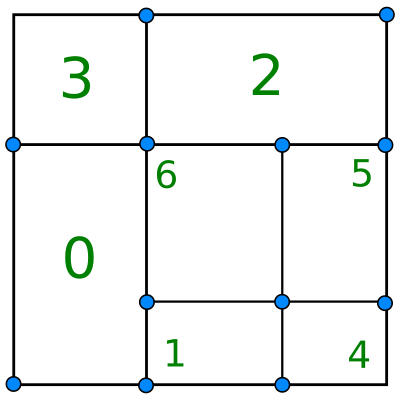
\includegraphics[width=0.6\linewidth]{fig/wpsl4.png}}
		\subfloat[\label{wpsl5}]{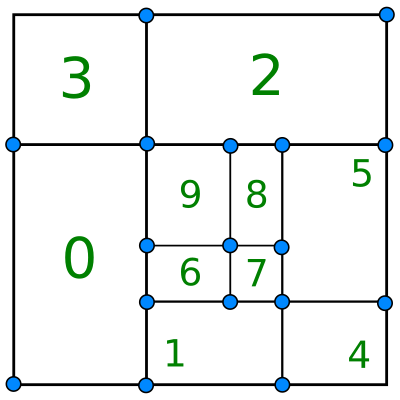
\includegraphics[width=0.6\linewidth]{fig/wpsl5.png}}
		\caption{How to add neighbors in adjacency list}
	\end{figure}
	
	Define a function \textit{is\_neighbor(node\_a, node\_b)} which will take two node as argument and return true if they are neighbors of each other (with/without periodic condition). It will be done using their coordinate and range of each arm.
	
	
	In fig (\ref{wpsl4}) node $6$ have neighbors $B=\{0,1,2,5\}$, therefore if four new node is placed (namely node $6,7,8,9$, note that label $6$ is recycled) in place of node $6$ then those node have a high chance of having $B$ as their neighbors. In fig (\ref{wpsl5}) we ask which nodes among $\{6,7,8,9\}$ are neighbors of $B=\{0,1,2,5\}$, if two nodes are neighbor then we put them in the adjacency list. 
	\begin{align}
		\text{old }, \quad 6 : \{0,1,2,5\} \\
		\text{new }, \quad 6 : \{0,1,7,9\} \\
		7 : \{1,6,8,5\} \\
		8 : \{2,5,7,9\} \\
		9 : \{0,2,6,8\}
	\end{align}
	
	\section{Finding Neighbor}
	There can be Two types of horizontal neighbors
	\begin{enumerate}
		\item Both top and bottom corner of one side of one of the rectangle is inside the range of the other rectangle fig (\ref{wpsl6}, \ref{wpsl8}).
		$y_2 < y_4$ and $y_1 > y_4$ for fig (\ref{wpsl6}).
		$y_4 < y_2$ and $y_3 > y_1$ for fig (\ref{wpsl8}).
		
		\item Only one corner is within range of the other rectangle fig (\ref{wpsl7}).
		
		 $y_2 > y_4 > y_1$. This is sufficient condition to be a neighbor.
		 
		 \item In case of periodic boundary, the right most box can be connected to the left most box. Horizontal periodicity can be checked using the condition $(x_1 + x_4) == 1$, since boundary $x$ coordinate can be either zero or one.
	\end{enumerate}

	Similar approach can be applied for vertical neighbors.
	\begin{figure}
		\centering
		\subfloat[\label{wpsl6}]{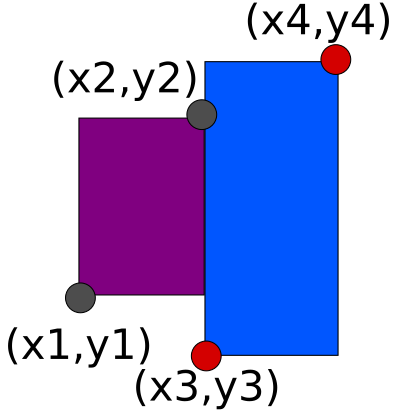
\includegraphics[width=0.4\linewidth]{fig/wpsl6.png}}
		\subfloat[\label{wpsl7}]{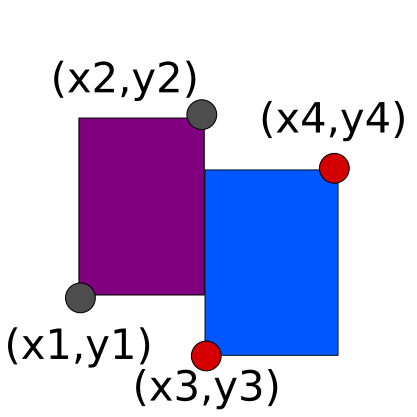
\includegraphics[width=0.4\linewidth]{fig/wpsl7.png}}
		\subfloat[\label{wpsl8}]{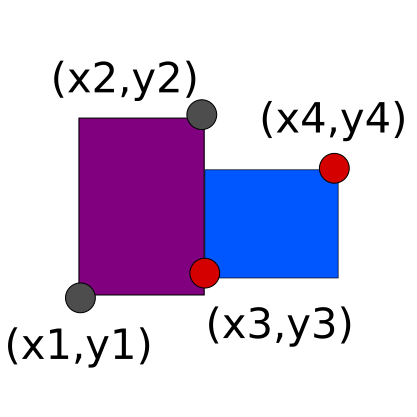
\includegraphics[width=0.4\linewidth]{fig/wpsl8.png}}
		\caption{Three types of horizontal neighbors. Note that $x_3 == x_2$ for all cases.}
	\end{figure}
	

\end{document}